%Este trabalho está licenciado sob a Licença Atribuição-CompartilhaIgual 4.0 Internacional Creative Commons. Para visualizar uma cópia desta licença, visite http://creativecommons.org/licenses/by-sa/4.0/deed.pt_BR ou mande uma carta para Creative Commons, PO Box 1866, Mountain View, CA 94042, USA.

\chapter{Perceptron}\label{cap_perceptron}
\thispagestyle{fancy}


\section{Unidade de Processamento}\label{cap_perceptron_sec_unit}

A \hl{\emph{unidade básica de processamento}} (neurônio artificial) que exploramos nestas notas \hl{é baseada no \emph{perceptron}} (consultemos a Fig. \ref{fig:perceptron}). \hl{Consiste na composição de uma \emph{função de ativação} $f:\mathbb{R}\to\mathbb{R}$ com a \emph{pré-ativação}}
\begin{align}
  \hleq{z} &\hleq{= \pmb{w}\cdot\pmb{x} + b} \\
    &= w_1x_1 + w_2x_2 + \cdots + w_nx_n + b
\end{align}
onde, $\pmb{x}\in\mathbb{R}^{n}$ é o \emph{vetor de entrada}, $\pmb{w}\in\mathbb{R}^{n}$ é o \emph{vetor de pesos} e $b\in\mathbb{R}$ é o \emph{\textit{bias}}. Escolhida uma função de ativação, a \emph{saída do neurônio} é dada por
\begin{align}
  \hleq y &\hleq := \mathcal{N}\left(\pmb{x};(\pmb{w},b)\right)\\
    &= f(z) = f(\pmb{w}\cdot\pmb{x} + b)
\end{align}
\hl{O treinamento (calibração) consiste em determinar os parâmetros $(\pmb{w}, b)$ de forma que o neurônio forneça as saídas $y$ esperadas com base em algum critério predeterminado}.

\begin{figure}[H]
  \centering
  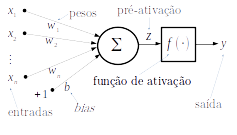
\includegraphics[width=0.7\textwidth]{./cap_perceptron/dados/fig_perceptron/fig}
  \caption{Esquema de um perceptron: unidade de processamento.}
  \label{fig:perceptron}
\end{figure}

Uma das vantagens deste modelo de neurônio é sua generalidade, i.e. pode ser aplicado a diferentes problemas. Na sequência, vamos aplicá-lo na resolução de um problema de classificação e noutro de regressão.


\subsection{Um problema de classificação}\label{cap_perceptron_ssec_classic}

\hl{Vamos desenvolver um perceptron que emule a operação $\land$ (e-lógico)}. I.e, receba como entrada dois valores lógicos $A_1$ e $A_2$ (V, verdadeiro ou F, falso) e forneça como saída o valor lógico $R = A_1 \land A_2$. Consultamos a seguinte tabela verdade:

\begin{center}
  \begin{tabular}{cc|c}
    $A_1$ & $A_2$ & R\\\hline
    V & V & V\\
    V & F & F\\
    F & V & F\\
    F & F & F\\\hline
  \end{tabular}
\end{center}


\subsubsection{Modelo}

Nosso \hl{\emph{modelo de neurônio}} será \hl{um perceptron com duas entradas $\pmb{x}\in \{-1,1\}^2$} e a função sinal
\begin{equation}
  f(z) = \sign(z) = \left\{
    \begin{array}{rr}
      1 &, z>0\\
      0 &, z=0\\
      -1 &, z<0
    \end{array}
\right.
\end{equation}
como função de ativação, i.e.
\begin{equation}
  \mathcal{N}\left(\pmb{x};(\pmb{w},b)\right) = \sign(\pmb{w}\cdot\pmb{x} + b),
\end{equation}
onde $\pmb{w}\in\mathbb{R}^2$ e $b\in\mathbb{R}$ são parâmetros a determinar.


\subsubsection{Pré-processamento}

Uma vez que nosso modelo recebe valores $\pmb{x}\in \{-1,1\}^2$ e retorna $y\in\{-1,1\}$, precisamos (pre)processar os dados do problema de forma a utilizá-lo. Uma forma, é assumir que todo valor negativo está associado ao valor lógico $F$ (falso) e positivo ao valor lógico $V$ (verdadeiro). Desta forma, os dados podem ser interpretados como na tabela abaixo.

\begin{center}
  \begin{tabular}{rr|c}
    $x_1$ & $x_2$ & $y$\\\hline
    1 & 1 & 1\\
    1 & -1 & -1\\
    -1 & 1 & -1\\
    -1 & -1 & -1\\\hline
  \end{tabular}
\end{center}
    
    
\subsubsection{Treinamento}

Agora, nos falta \hl{treinar nosso neurônio para fornecer o valor de $y$ esperado para cada dada entrada $\pmb{x}$}. Isso \hl{consiste em um método para escolhermos os parâmetros $(\pmb{w},b)$} que sejam adequados para esta tarefa. Vamos explorar mais sobre isso na sequência do texto e, aqui, apenas escolhemos
\begin{gather}
  \pmb{w} = [1, 1]\\
  b = -1
\end{gather}
Com isso, nosso perceptron é
\begin{equation}
  \mathcal{N}(\pmb{x}) = \sign(x_1 + x_2 - 1)
\end{equation}
Verifique que ele satisfaz a tabela verdade acima!


\subsubsection{Implementação}

% {./cap_perceptron/dados/py_perceptron/main.py}
\begin{lstlisting}[caption=perceptron.py, label=cap_perceptron_sec_unit:cod:perceptron]
import torch

# modelo
class Perceptron(torch.nn.Module):
    def __init__(self):
        super().__init__()
        self.linear = torch.nn.Linear(2,1)

    def forward(self, x):
        z =  self.linear(x)
        y = torch.sign(z)
        return y

model = Perceptron()
W = torch.Tensor([[1., 1.]])
b = torch.Tensor([-1.])
with torch.no_grad():
    model.linear.weight = torch.nn.Parameter(W)
    model.linear.bias = torch.nn.Parameter(b)

# dados de entrada
X = torch.tensor([[1., 1.],
                  [1., -1.],
                  [-1., 1.],
                  [-1., -1.]])

print(f"\nDados de entrada\n{X}")


# forward (aplicação do modelo)
y = model(X)

print(f"Valores estimados\n{y}")
\end{lstlisting}

\subsubsection{Interpretação geométrica}

Empregamos o seguinte modelo de neurônio
\begin{equation}
  \mathcal{N}\left(\pmb{x};(\pmb{w},b)\right) = \sign(w_1x_1 + w_2x_2 + b)
\end{equation}
Observamos que
\begin{equation}
  w_1x_1 + w_2x_2 + b = 0
\end{equation}
corresponde à equação geral de uma reta no plano $\tau: x_1\times x_2$. Esta reta divide o plano em dois semiplanos
\begin{align}
  \tau^+ = \{\pmb{x}\in\mathbb{R}^2: w_1x_1 + w_2x_2 + b > 0\}\\
  \tau^- = \{\pmb{x}\in\mathbb{R}^2: w_1x_1 + w_2x_2 + b < 0\}
\end{align}
O primeiro está na direção do vetor normal a reta $\pmb{n} = (w_1, w_2)$ e o segundo na sua direção oposta. Com isso, o problema de treinar nosso neurônio para nosso problema de classificação consiste em encontrar a reta
\begin{equation}
  w_1x_1 + w_2x_2 + b = 0
\end{equation}
de forma que o ponto $(1,1)$ esteja no semiplano positivo $\tau^+$ e os demais pontos no semiplano negativo $\tau^-$. Consulte a Figura \ref{fig:class_e}.

\begin{figure}[H]
  \centering
  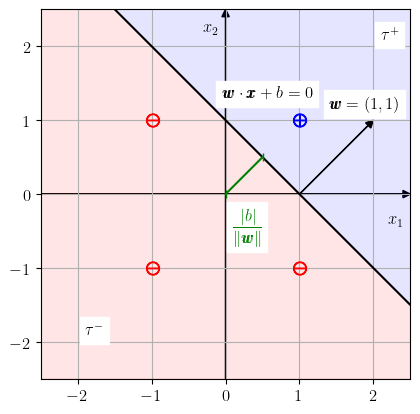
\includegraphics[width=0.7\textwidth]{./cap_perceptron/dados/fig_class_e/main}
  \caption{Interpretação geométrica do perceptron aplicado ao problema de classificação relacionado à operação lógica $\land$ (e-lógico).}
  \label{fig:class_e}
\end{figure}

\subsubsection{Algoritmo de treinamento: perceptron}

O \hl{algoritmo de treinamento perceptron permite calibrar os pesos de um neurônio para fazer a classificação de dados linearmente separáveis}. Trata-se de um algoritmo para o \hl{\emph{treinamento supervisionado}} de um neurônio, i.e. \hl{a calibração dos pesos é feita com base em um dado \emph{conjunto de amostras de treinamento}}.

Seja dado um \emph{conjunto de treinamento} $\{\pmb{x}^{(s)},y^{(s)}\}_{s=1}^{n_s}$, onde $n_s$ é o número de amostras. O algoritmo consiste no seguinte:
\begin{enumerate}
\item $\pmb{w} \leftarrow\pmb{0}$, $b \leftarrow 0$.
\item Para $e \leftarrow 1,\dotsc, n_e$:
  \begin{enumerate}
  \item Para $s \leftarrow 1,\dotsc, n_s$:
    \begin{enumerate}
    \item Se $y^{(s)}\mathcal{N}\left(\pmb{x}^{(s)}\right) \leq 0$:
      \begin{enumerate}
      \item $\pmb{w} \leftarrow \pmb{w}+y^{(s)}\pmb{x}^{(s)}$
      \item $b \leftarrow b + y^{(s)}$
      \end{enumerate}
    \end{enumerate}
  \end{enumerate}
\end{enumerate}
onde, $n_e$ é um dado número de épocas\footnote{Número de vezes que as amostrar serão percorridas para realizar a correção dos pesos.}.

% \lstinputlisting[caption=perceptron\_train.py, label=cap_perceptron_sec_unit:cod:perceptron_train]{./cap_perceptron/dados/py_perceptron_train/main.py}
\begin{lstlisting}
import torch

# modelo

class Perceptron(torch.nn.Module):
    def __init__(self):
        super().__init__()
        self.linear = torch.nn.Linear(2,1)

    def forward(self, x):
        z =  self.linear(x)
        y = torch.sign(z)
        return y

model = Perceptron()
with torch.no_grad():
    W = model.linear.weight
    b = model.linear.bias

# dados de treinamento
X_train = torch.tensor([[1., 1.],
                  [1., -1.],
                  [-1., 1.],
                  [-1., -1.]])
y_train = torch.tensor([1., -1., -1., -1.]).reshape(-1,1)

## número de amostras
ns = y_train.size(0)

print("\nDados de treinamento")
print("X_train =")
print(X_train)
print("y_train = ")
print(y_train)

# treinamento

## num max épocas
nepochs = 100

for epoch in range(nepochs):

    # update
    not_updated = True
    for s in range(ns):
        y_est = model(X_train[s:s+1,:])
        if (y_est*y_train[s] <= 0.):
            with torch.no_grad():
                W += y_train[s]*X_train[s,:]
                b += y_train[s]
                not_updated = False

    if (not_updated):
        print('Training ended.')
        break


# verificação
print(f'W =\n{W}')
print(f'b =\n{b}')
y = model(X_train)
print(f'y =\n{y}')
\end{lstlisting}

\subsection{Problema de regressão}\label{cap_perceptron_ssec_regr}

Vamos \hl{treinar um perceptron para resolver o problema de regressão linear} para os seguintes dados

\begin{center}
  \begin{tabular}{l|ll}
    s & $x^{(s)}$ & $y^{(s)}$\\\hline
    1 & 0.5 & 1.2\\
    2 & 1.0 & 2.1\\
    3 & 1.5 & 2.6\\
    4 & 2.0 & 3.6\\\hline
  \end{tabular}
\end{center}

\subsubsection{Modelo}

Vamos determinar o perceptron\footnote{Escolhendo $f(z)=z$ como função de ativação.}
\begin{equation}\label{eq:percep_regr}
  \tilde{y} = \mathcal{N}(x; (w, b)) = wx + b
\end{equation}
que melhor se ajusta a este conjunto de dados $\left\{(x^{(s)}, y^{(s)})\right\}_{s=1}^{n_s}$, $n_s=4$.

\subsubsection{Treinamento}

A \hl{ideia é que o perceptron seja tal que minimize o erro quadrático médio (MSE, do inglês, \textit{Mean Squared Error})}, i.e.
\begin{equation}\label{eq_percep:regr_prob}\hleq
  \min_{w,b}\frac{1}{n_s}\sum_{s=1}^{n_s}\left(\tilde{y}^{(s)}-y^{(s)}\right)^2
\end{equation}
Vamos denotar a \hl{\emph{função erro}} (em inglês, \textit{loss function}) por
\begin{align}\label{eq:eqm}
  \varepsilon(w,b) &:= \frac{1}{n_s}\sum_{s=1}^{n_s}\left(\tilde{y}^{(s)}-y^{(s)}\right)^2\\
                   &= \frac{1}{n_s}\sum_{s=1}^{n_s}\left(wx^{(s)}+b-y^{(s)}\right)^2
\end{align}

Observamos que o problema \eqref{eq_percep:regr_prob} é equivalente a um problema linear de \href{https://notaspedrok.com.br/notas/MatematicaNumerica/cap_ajuste_sec_prob_lin.html}{mínimos quadrados}. A solução é obtida resolvendo-se a equação normal\footnote{Consulte o Exercício \ref{exer_percep:sol_mq}.}
\begin{equation}\label{eq_percep:sol_mq}
  M^TM\pmb{c} = M^T\pmb{y},
\end{equation}
onde $\pmb{c} = (w, p)$ é o vetor dos parâmetros a determinar e $M$ é a matriz $n_s\times 2$ dada por
\begin{equation}
  M =
  \begin{bmatrix}
    \pmb{x} & \pmb{1}
  \end{bmatrix}
\end{equation}

\subsubsection{Implementação}

% lstinputlisting[caption=perceptron\_mq.py, label=cap_perceptron_sec_unit:cod:perceptron_mq]{./cap_perceptron/dados/py_perceptron_mq/main.py}
\begin{lstlisting}[caption=perceptron\_mq.py, label=cap_perceptron_sec_unit:cod:perceptron_mq]
import torch

# modelo

class Perceptron(torch.nn.Module):
    def __init__(self):
        super().__init__()
        self.linear = torch.nn.Linear(1,1)

    def forward(self, x):
        z =  self.linear(x)
        return z

model = Perceptron()
with torch.no_grad():
    W = model.linear.weight
    b = model.linear.bias

# dados de treinamento
X_train = torch.tensor([0.5,
                        1.0,
                        1.5,
                        2.0]).reshape(-1,1)
y_train = torch.tensor([1.2,
                        2.1,
                        2.6,
                        3.6]).reshape(-1,1)

## número de amostras
ns = y_train.size(0)

print("\nDados de treinamento")
print("X_train =")
print(X_train)
print("y_train = ")
print(y_train)

# treinamento

## matriz
M = torch.cat((X_train,
               torch.ones((ns,1))), dim=1)
## solucão M.Q.
c = torch.linalg.lstsq(M, y_train)[0]
with torch.no_grad():
    W = c[0]
    b = c[1]

# verificação
print(f'W =\n{W}')
print(f'b =\n{b}')
y = model(X_train)
print(f'y =\n{y}')
\end{lstlisting}

\subsubsection{Resultado}

Nosso perceptron corresponde ao modelo
\begin{equation}
  \mathcal{N}(x; (w,b)) = wx + b
\end{equation}
com os pesos treinados $w = 1.54$ e $b = 0.45$. Ele corresponde à reta que melhor se ajusta ao conjunto de dados de $\left\{x^{(s)}, y^{(s)}\right\}$. Consulte a Figura \ref{fig:percep_mq}.

\begin{figure}[H]
  \centering
  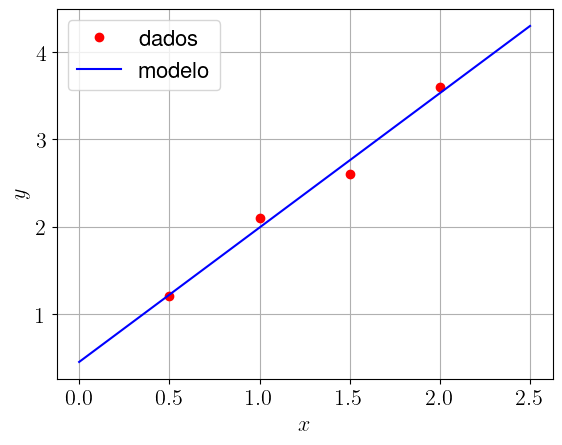
\includegraphics[width=0.7\textwidth]{./cap_perceptron/dados/fig_percep_mq/main}
  \caption{Interpretação geométrica do perceptron aplicado ao problema de regressão linear.}
  \label{fig:percep_mq}
\end{figure}

\subsection{Exercícios}

\begin{exer}
  Crie um Perceptron que emule a operação lógica do $\lor$ (\texttt{ou-lógico}).
  \begin{center}
    \begin{tabular}{cc|c}
      $A_1$ & $A_2$ & $A_1\lor A_2$\\\hline
      V & V & V\\
      V & F & V\\
      F & V & V\\
      F & F & F\\\hline
    \end{tabular}
  \end{center}
\end{exer}

\begin{exer}
  Busque criar um Perceptron que emule a operação lógica do $\texttt{xor}$.
  \begin{center}
    \begin{tabular}{cc|c}
      $A_1$ & $A_2$ & $A_1\texttt{ xor }A_2$\\\hline
      V & V & F\\
      V & F & V\\
      F & V & V\\
      F & F & F\\\hline
    \end{tabular}
  \end{center}
  É possível? Justifique sua resposta.
\end{exer}

\begin{exer}\label{exer:eqm_convexa}
  Assumindo o modelo de neurônio \eqref{eq:percep_regr}, mostre que \eqref{eq:eqm} é função convexa.
\end{exer}
\begin{resp}
  Dica: verifique que sua matriz hessiana é positiva definida.
\end{resp}

\begin{exer}\label{exer_percep:sol_mq}
  Mostre que a solução do problema \eqref{eq_percep:regr_prob} é dada por \eqref{eq_percep:sol_mq}.
\end{exer}
\begin{resp}
  Dica: consulte a ligação \href{https://notaspedrok.com.br/notas/MatematicaNumerica/cap_ajuste_sec_prob_lin.html}{Notas de Aula: Matemática Numérica: 7.1 Problemas lineares}.
\end{resp}

\begin{exer}
  Crie um Perceptron com função de ativação $f(x)=\tanh(x)$ que melhor se ajuste ao seguinte conjunto de dados:
  \begin{center}
  \begin{tabular}{l|rr}
    s & $x^{(s)}$ & $y^{(s)}$\\\hline
    1 & -1,0 & -0,8 \\
    2 & -0,7 & -0,7 \\
    3 & -0,3 & -0,5 \\
    4 &  0,0 & -0,4 \\
    5 &  0,2 & -0,2 \\
    6 &  0,5 &  0,0 \\
    7 &  1,0 &  0,3 \\\hline
  \end{tabular}
\end{center}
\end{exer}

\section{Algoritmo de Treinamento}\label{cap_percepton_sec_train}

Na seção anterior, desenvolvemos dois modelos de neurônios para problemas diferentes, um de classificação e outro de regressão. Em cada caso, utilizamos algoritmos de treinamento diferentes. Agora, vamos estudar algoritmos de treinamentos mais gerais\footnote{Aqui, vamos explorar apenas algoritmos de treinamento supervisionado.}, que podem ser aplicados a ambos os problemas.

Ao longo da seção, vamos considerar o \hl{\emph{modelo}} de neurônio
\begin{equation}
  \hleq \tilde{y} = \mathcal{N}\left(\pmb{x}; (\pmb{w}, b)\right) = f\underbrace{(\pmb{w}\cdot\pmb{x} + b)}_{z},
\end{equation}
com dada função de ativação $f:\mathbb{R}\to\mathbb{R}$, sendo os vetores de entrada $\pmb{x}$ e dos pesos $\pmb{w}$ de tamanho $n_{in}$. A pré-ativação do neurônio é denotada por
\begin{equation}
  z := \pmb{w}\cdot\pmb{x} + b
\end{equation}

\hl{Fornecido um \emph{conjunto de treinamento}} $\left\{\left(\pmb{x}^{(s)}, y^{(s)}\right)\right\}_1^{n_s}$, com $n_s$ amostras, \hl{o objetivo é calcular os parâmetros $(\pmb{w}, b)$ que minimizam a \emph{função erro quadrático médio}}
\begin{align}\label{eq:percep_mse}
  \hleq\varepsilon(\pmb{w}, b) &\hleq := \frac{1}{n_s}\sum_{s=1}^{n_s}\left(\tilde{y}^{(s)} - y^{(s)}\right)^2\\
                          &= \frac{1}{n_s}\sum_{s=1}^{n_s}\varepsilon^{(s)}
\end{align}
onde $\tilde{y}^{(s)} = \mathcal{N}\left(\pmb{x}^{(s)}; (\pmb{w}, b)\right)$ é o \emph{valor estimado} pelo modelo e $y^{(s)}$ é o \emph{valor esperado} para a $s$-ésima amostra. A função erro para a $s$-ésima amostra é
\begin{equation}\hleq
  \varepsilon^{(s)} := \left(\tilde{y}^{(s)} - y^{(s)}\right)^2.
\end{equation}

Ou seja, \hl{o treinamento consiste em resolver o seguinte \emph{problema de otimização}}
\begin{equation}\hleq
  \min_{(\pmb{w}, b)}\varepsilon(\pmb{w}, b)
\end{equation}

Para resolver este problema de otimização, vamos empregar o Método do Gradiente Descendente.

\subsection{Método do Gradiente Descendente}

\hl{O \emph{Método do Gradiente Descendente} (GD, em inglês, \textit{Gradiente Descent Method}) é um }\href{https://notaspedrok.com.br/notas/MatematicaNumericaAvancada/cap_otimizacao_sec_minimi.html}{\hl{método de declive}}. Aplicado ao nosso modelo de Perceptron consiste no seguinte algoritmo:
\begin{enumerate}
\item $(\pmb{w}, b)$ aproximação inicial.
\item Para $e\leftarrow 1, \dotsc, n_e$:
  \begin{enumerate}
  \item $\displaystyle (\pmb{w}, b) \leftarrow (\pmb{w}, b) - l_r\frac{\p\varepsilon}{\p (\pmb{w}, b)}$
  \end{enumerate}
\end{enumerate}
onde, $n_e$ é o \hl{\emph{número de épocas}}, $l_r$ é uma dada \hl{\emph{taxa de aprendizagem} ($l_r$, do inglês, \textit{learning rate})} e o \hl{\emph{gradiente}} é
\begin{equation}\hleq
  \frac{\p\varepsilon}{\p (\pmb{w}, b)} := \left(\frac{\p\varepsilon}{\p w_1}, \dotsc, \frac{\p\varepsilon}{\p w_{n_{in}}}, \frac{\p\varepsilon}{\p b}\right)
\end{equation}

O cálculo do gradiente para os pesos $\pmb{w}$ pode ser feito como segue
\begin{align}
  \frac{\p\varepsilon}{\p \pmb{w}} &= \frac{\p}{\p\pmb{w}}\left[\frac{1}{n_s}\sum_{s=1}^{n_s}\varepsilon^{(s)}\right]\\
                                   &= \frac{1}{ns}\sum_{s=1}^{ns}\frac{\p\varepsilon^{(s)}}{\p\tilde{y}^{(s)}}\frac{\p\tilde{y}^{(s)}}{\p\pmb{w}}\\
  {\color{blue}\frac{\p\varepsilon}{\p \pmb{w}}} &{\color{blue}= \frac{1}{ns}\sum_{s=1}^{ns}\frac{\p\varepsilon^{(s)}}{\p\tilde{y}^{(s)}}\frac{\p\tilde{y}^{(s)}}{\p z^{(s)}}\frac{\p z^{(s)}}{\p\pmb{w}}}
\end{align}
Observando que
\begin{gather}
  \frac{\p\varepsilon^{(s)}}{\p\tilde{y}^{(s)}} = 2\left(\tilde{y}^{(s)} - y^{(s)}\right)\\
  \frac{\p\tilde{y}^{(s)}}{\p z^{(s)}} = f'\left(z^{(s)}\right)\\
  \frac{\p z^{(s)}}{\p\pmb{w}} = \pmb{x}^{(s)}
\end{gather}
obtemos
\begin{equation}
  \frac{\p\varepsilon}{\p \pmb{w}} = \frac{1}{n_s}\sum_{s=1}^{n_s}2\left(\tilde{y}^{(s)}-y^{(s)}\right)f'\left(z^{(s)}\right)\pmb{x}^{(s)}
\end{equation}
\begin{align}
  {\color{blue}\frac{\p\varepsilon}{\p b}} &{\color{blue}= \frac{1}{ns}\sum_{s=1}^{ns}\frac{\p\varepsilon^{(s)}}{\p\tilde{y}^{(s)}}\frac{\p\tilde{y}^{(s)}}{\p z^{(s)}}\frac{\p z^{(s)}}{\p b}}\\
  \frac{\p\varepsilon}{\p b} &= \frac{1}{n_s}\sum_{s=1}^{n_s}2\left(\tilde{y}^{(s)}-y^{(s)}\right)f'\left(z^{(s)}\right)\cdot 1
\end{align}

\subsubsection{Aplicação: Problema de Classificação}

Na Subseção \ref{cap_perceptron_ssec_classic}, \hl{treinamos um Perceptron para o problema de classificação do e-lógico}. A função de ativação $f(x) = \sign(x)$ não é adequada para a aplicação do Método GD, pois $f'(x) \equiv 0$ para $x\neq 0$. Aqui, vamos usar
\begin{equation}
  f(x) = \tanh(x).
\end{equation}

% \lstinputlisting[caption=perceptron\_gd.py, label=cap_perceptron_sec_train:cod:perceptron_gd]{./cap_perceptron/dados/py_perceptron_gd/main.py}
\begin{lstlisting}[caption=perceptron\_gd.py, label=cap_perceptron_sec_train:cod:perceptron_gd]
import torch

# modelo

class Perceptron(torch.nn.Module):
    def __init__(self):
        super().__init__()
        self.linear = torch.nn.Linear(2,1)

    def forward(self, x):
        z =  self.linear(x)
        y = torch.tanh(z)
        return y

model = Perceptron()

# treinamento

## optimizador
optim = torch.optim.SGD(model.parameters(), lr=1e-1)

## função erro
loss_fun = torch.nn.MSELoss()

## dados de treinamento
X_train = torch.tensor([[1., 1.],
                  [1., -1.],
                  [-1., 1.],
                  [-1., -1.]])
y_train = torch.tensor([1., -1., -1., -1.]).reshape(-1,1)

print("\nDados de treinamento")
print("X_train =")
print(X_train)
print("y_train = ")
print(y_train)

## num max épocas
nepochs = 5000
tol = 1e-3

for epoch in range(nepochs):

    # forward
    y_est = model(X_train)

    # erro
    loss = loss_fun(y_est, y_train)

    print(f'{epoch}: {loss.item():.4e}')

    # critério de parada
    if (loss.item() < tol):
        break

    # backward
    optim.zero_grad()
    loss.backward()
    optim.step()


# verificação
y = model(X_train)
print(f'y_est = {y}')
\end{lstlisting}

\subsection{Método do Gradiente Estocástico}

O \hl{\emph{Método do Gradiente Estocástico}} (SGD, do inglês, \textit{Stochastic Gradient Descent Method}) é um variação do Método GD. \hl{A ideia é atualizar os parâmetros do modelo com base no gradiente do erro de cada amostra (ou um subconjunto de amostras)}. A estocasticidade é obtida da randomização com que as amostras são escolhidas a cada época. O algoritmos consiste no seguinte:
\begin{enumerate}[1.]
\item \pmb{w}, b aproximações inicial.
\item Para $e\leftarrow 1,\dotsc, n_e$:
  \begin{enumerate}[1.1.]
  \item Para $s\leftarrow \texttt{random}(1,\dotsc, n_s)$:
    \begin{equation}
      (\pmb{w}, b) \leftarrow (\pmb{w}, b) - l_r\frac{\p\varepsilon^{(s)}}{\p(\pmb{w}, b)}
    \end{equation}
  \end{enumerate}
\end{enumerate}

\subsubsection{Aplicação: Problema de Classificação}

% \lstinputlisting[caption=perceptron\_sgd.py, label=cap_perceptron_sec_train:cod:perceptron_sgd]{./cap_perceptron/dados/py_perceptron_sgd/main.py}
\begin{lstlisting}[caption=perceptron\_sgd.py, label=cap_perceptron_sec_train:cod:perceptron_sgd]
import torch
import numpy as np

# modelo

class Perceptron(torch.nn.Module):
    def __init__(self):
        super().__init__()
        self.linear = torch.nn.Linear(2,1)

    def forward(self, x):
        z =  self.linear(x)
        y = torch.tanh(z)
        return y

model = Perceptron()

# treinamento

## optimizador
optim = torch.optim.SGD(model.parameters(), lr=1e-1)

## função erro
loss_fun = torch.nn.MSELoss()

## dados de treinamento
X_train = torch.tensor([[1., 1.],
                  [1., -1.],
                  [-1., 1.],
                  [-1., -1.]])
y_train = torch.tensor([1., -1., -1., -1.]).reshape(-1,1)

## num de amostras
ns = y_train.size(0)

print("\nDados de treinamento")
print("X_train =")
print(X_train)
print("y_train = ")
print(y_train)

## num max épocas
nepochs = 5000
tol = 1e-3

for epoch in range(nepochs):

    # forward
    y_est = model(X_train)

    # erro
    loss = loss_fun(y_est, y_train)

    print(f'{epoch}: {loss.item():.4e}')

    # critério de parada
    if (loss.item() < tol):
        break

    # backward
    for s in torch.randperm(ns):
        loss_s = (y_est[s,:] - y_train[s,:])**2
        optim.zero_grad()
        loss_s.backward()
        optim.step()
        y_est = model(X_train)


# verificação
y = model(X_train)
print(f'y_est = {y}')
\end{lstlisting}


\subsection{Exercícios}

\begin{exer}
  Calcule a derivada da função de ativação
  \begin{equation}
    f(x) = \tanh(x).
  \end{equation}
\end{exer}
\begin{resp}
  $(\tanh x)' = 1 - \tanh^2 x$
\end{resp}

\begin{exer}
  Crie um Perceptron para emular a operação lógica $\land$ (\texttt{e-lógico}). No treinamento, use como otimizador:
  \begin{enumerate}[a)]
  \item Método GD.
  \item Método SGD.
  \end{enumerate}
\end{exer}

\begin{exer}
  Crie um Perceptron para emular a operação lógica $\lor$ (\texttt{ou-lógico}). No treinamento, use como otimizador:
  \begin{enumerate}[a)]
  \item Método GD.
  \item Método SGD.
  \end{enumerate}
\end{exer}

\begin{exer}
  Crie um Perceptron que se ajuste ao seguinte conjunto de dados:
  \begin{center}
    \begin{tabular}{l|ll}
      s & $x^{(s)}$ & $y^{(s)}$\\\hline
      1 & 0.5 & 1.2\\
      2 & 1.0 & 2.1\\
      3 & 1.5 & 2.6\\
      4 & 2.0 & 3.6\\\hline
    \end{tabular}
  \end{center}
  No treinamento, use como otimizador:
  \begin{enumerate}[a)]
  \item Método GD.
  \item Método SGD.
  \end{enumerate}  
\end{exer}
